% !TEX root = thesis.tex
\graphicspath{{./figures/}}

%%%%%%%%%%%%%%%%%%%%%%%%
\chapter{Implementation}
%%%%%%%%%%%%%%%%%%%%%%%%

\section{Iterative Approach}
\label{sec:iterative_approach}

\subsection{Simple Iterative Approach}

In order to come up with an algorithm to resolve delegations, we first describe intuitively what the algorithm should do. It may make sense to think about power as a liquid flowing through the graph. Each delegator is a "source", and power flows from its source between nodes until it eventually ends in a sink. If a delegator A delegates half their vote to B and the other half to other nodes, half of A's power should flow to B. An algorithm should thus add 0.5 to Bs power, and remove it from A. If B is a sink, the algorithm is done resolving this delegation. However,  B may not be a sink, in which case, the power continues to flow further, to B's delegates. An algorithm would need to iterate over the graph multiple times, until an equilibrium has been reached, where all power in the graph has flown into a sink. \Cref{alg:iterative_simple} shows such an algorithm drafted in pseudocode. Each iteration, a snapshot of the power's of each node is taken, and the reassignments of power are based on this snapshot\footnotemark.  

\footnotetext{If the algorithm forwent the use of such a snapshot, it would lead to inconsistencies in the edge case of a self-delegation of weight less than 1, since the self-delegator's power would change in the middle of reassigning the power. }

Another valid approach would be a queue-approach, where the algorithm pops node off a queue and delegates their power, and each delegate of this node gets re-added to the queue. A sweeping method treating the entire graph at once was chosen due to its increased simplicity and runtime analysis.

\begin{algorithm} [H]
 \caption{Iterative Algorithm}\label{alg:iterative_simple}
\begin{algorithmic}[1]
\State // Initialize each node’s power to 1.0  
\ForAll{\(v \in \texttt{nodes}\)}
    \State \(\texttt{powers}[v] \gets 1.0\)
\EndFor
\Repeat
    \State \(\texttt{prev\_powers} \gets \texttt{powers}.\texttt{copy}()\)  \Comment{snapshot of previous iteration}
    \ForAll{\(v \in \texttt{nodes}\)}
        \State // For each incoming delegation \((u \to v)\), move \(w_{uv}\times\) previous power of u
        \ForAll{\((u, w) \in \texttt{delegations}[v]\)}
            \State \(\delta \gets w \times \texttt{prev\_powers}[u]\) \label{alg:iterative_simple_delta_assignment}
            \State \(\texttt{powers}[u] \;-\!=\; \delta\) \label{alg:iterative_simple_remove_delta}
            \State \(\texttt{powers}[v] \;+\!=\; \delta\) \label{alg:iterative_simple_add_delta}
        \EndFor
    \EndFor
\Until{\(\texttt{prev\_powers} = \texttt{powers}\)} \label{alg:iterative_simple_termination_cond}\Comment{a steady state has been reached}
\end{algorithmic}
\end{algorithm}

The following notation will be used throughout the next sections.

$G = (V, E)$ is a well-formed delegation graph, with $V = D \dot\bigcup S$, where D is the set of delegators and S is the set of sinks.

Let $p_v^{(i)}, i \in \mathbb{N}_0$ be \texttt{powers}[v] after the $i$-th iteration of the repeat-until loop, with $p_v^{(0)}$ being the initial power of a node before the first iteration has started. Using this notation, our termination condition for the repeat-until loop at \cref{alg:iterative_simple_termination_cond} of \cref{alg:iterative_simple} is: $\forall v \in V: p_v^{(i-1)} = p_v^{(i)}$

Let $P_D^{(i)} = \sum_{d \in D} p_d^{(i)}$ and $P_S^{(i)} = \sum_{s \in S} p_s^{(i)}$ be the sums of all delegators and all sinks after each iteration.

Let $\delta_{(u, v, w)}^{(i)}$ be the delta assigned in \cref{alg:iterative_simple} at \cref{alg:iterative_simple_delta_assignment} during the $i$th iteration.

\subsubsection{Conservation of Power}

This algorithm conserves power.

\begin{theorem}
\label{theo:iterative_cons_of_power}
Given a well-formed delegation graph, in \cref{alg:iterative_simple}, $P_t^{(i)} = P_D^{(i)} + P_S^{(i)}$ is equal to $|V|$ for any $i \in \mathbb{N}_0$.
\end{theorem}
\begin{proof}

We prove the theorem inductively. When $i = 0$ (before the first iteration), each node is assigned a power of 1. So 

\[
\forall v \in V: p_v^{(i)} = 1 \implies P_t^{(0)} = |V|
\]

Assume that for a $k \in \mathbb{N}_0: P_t^{(k)} = |V|$. During iteration $k+1$, the algorithm will iterate over all delegations, and for each $(u, v, w) \in E$, it will remove some $\delta_{(u, v, w)}^{(k+1)}$ from node \texttt{u} in \cref{alg:iterative_simple_remove_delta}, but add this same amount to node \texttt{v} in \cref{alg:iterative_simple_add_delta}. Since the delegation graph is well formed, the outgoing weights of any delegator add up to 1, so for all delegators $u \in D$, the total amount of power they delegate away during iteration $k+1$ adds up to the power they held in iteration $k$.

\begin{align*}
\sum_{(u, v, w) \in E} \delta_{(u, v, w)}^{(k+1)} &=  \sum_{(u, v, w) \in E} wp_u^{(k)} \\
&= p_u^{(k)}  \sum_{(u, v, w) \in E} w \\
&= p_u^{(k)} \cdot 1 \\
&= p_u^{(k)}
\end{align*}

Thus, throughout the iteration of the outer loop, any delegator $u$ only ever moves power it already has, and for each "moving around" of power, conservation is guaranteed since any power subtracted from a delegator is re-added to the delegate. This means that power is only ever moved around, but not lost, and $P_t^{(k+1)} = |V|$. 

By the principles of induction, the assumption holds for any $i \in \mathbb{N}_0$
\end{proof}

\subsubsection{Termination}

Given a well formed delegation graph, this algorithm doesn't necessarily terminate, as shown by the following lemmata and theorem.

First, we prove that a sink's power can't shrink, since there is no outgoing edge going out of a sink.

\begin{lemma}\label{lem:sink_non_shrink}
$\forall s \in S: p_s^{(i)} \ge p_s^{(i-1)}$ 
\end{lemma}
\begin{proof}
Assume $p_s^{(i)} < p_s^{(i-1)}$. The power that left $s$ needs to have gone somewhere, since the algorithm conserves power. This implies, that there is a delegation $(s, v, w) \in E$ such that $\exists \delta > 0: \delta \gets w * p_s^{(i-1)}$. This contradicts our definition of a well-formed liquid delegation graph, since any sink can not have any outgoing edges.
\end{proof}

Next, we prove that if a node's power is 0, all its delegator's powers must have been 0 after the previous iteration
\begin{lemma}\label{lem:simple_iterative_empty_node}
$p_v^{(i)} = 0 \implies \forall (u, v, w) \in E: p_u^{(i - 1)} = 0$. 
\end{lemma}
\begin{proof} Assume $p_v^{(i)} = 0$, but $\exists (u, v, w) \in E: p_u^{(i-1)} > 0$

Let $d \in \mathbb{R}_{0}$ be any additional power a node receives, that is not explicitly mentioned.

\[
p_u^{(i-1)} > 0 \implies \delta_{(u, v, w)}^{(i)} > 0 \implies p_v^{(i)} = \delta_{(u, v, w)}^{(i)} + d \implies p_v^{(i)} > 0 \lightning
\]

\end{proof}

Next, we prove that the algorithm terminates at iteration $i+1$ exactly when $P_D^{(i)} = 0$.

\begin{lemma}\label{lem:simple_alg_terminates}
 $p_v^{(i)} = p_v^{(i+1)} \forall v \in V \Leftrightarrow$ $P_D^{(i)} = 0$.
\end{lemma}
\begin{proof}

\begin{align*}
	P_D^{(i)} = 0 
	&\Leftrightarrow p_d^{(i)} = 0, \forall d \in D \\
	&\Leftrightarrow \not\exists (d, v, w) \in E: \delta_{(d, v, w)}^{(i+1)} > 0  &&\text{($\delta$ of a node with power 0 is 0)}\\
	&\Leftrightarrow p_v^{(i)} = p_v^{(i+1)} \forall v \in V \qed  &&\text{($p_v$ doesn't change if zero is added to it)}
\end{align*}
\end{proof}

\begin{theorem}\label{alg:iterative_alg_doesnt_terminate}
Given a well-formed delegation graph, \cref{alg:iterative_simple} may not terminate.
\end{theorem}
\begin{proof} Assume the algorithm terminates on a well-formed delegation graph..

Take the following well formed delegation graph $G = (S \dot\bigcup D, E)$with $S =\{C\}$ and $D = \{A, B\}$. B delegates half their vote to A, and half their vote to C, while A delegates its entire vote back to B. Since the algorithm terminates, there must be an $i \in \mathbb{N}$ such that $P_D^{(i)} = 0$. 

\begin{figure}[h]
    \centering
    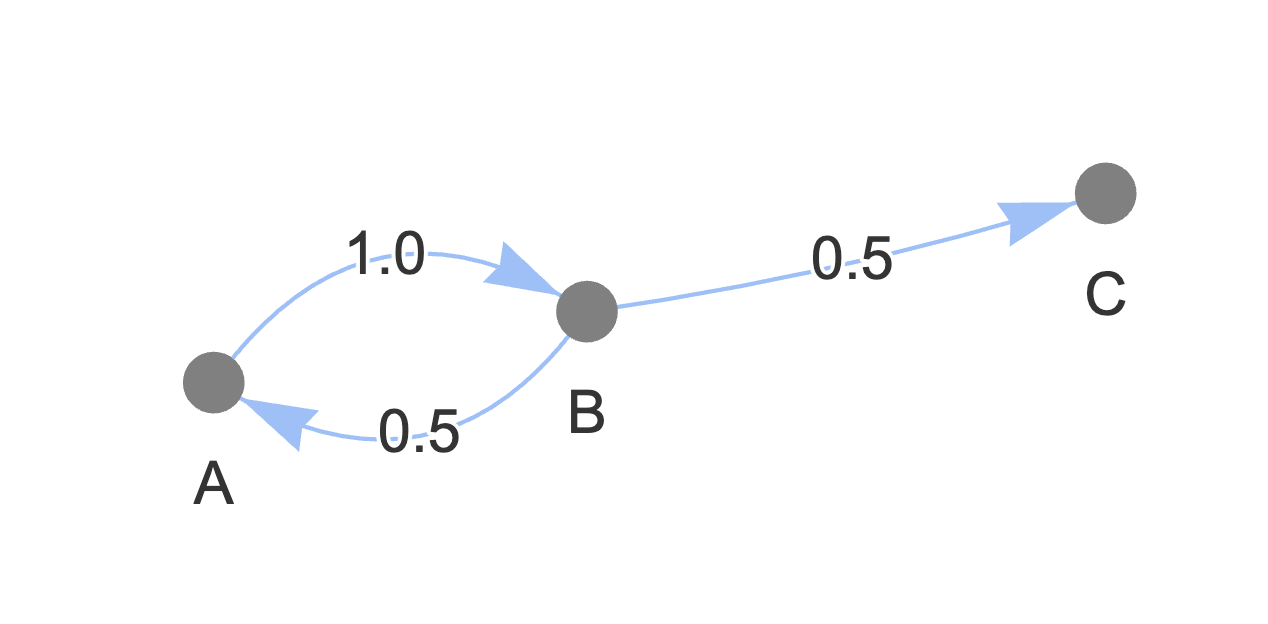
\includegraphics[width=0.4\textwidth]{small_cycle_graph}
    \caption{Delegation graph with a cycle.}
    \label{fig:small_cycle_graph}
\end{figure}


Both (B, A, 0.5) and (A, B, 1) $\in E$, so A is a predecessor of B, and B is a predecessor of A, thus B is its own predecessor.

\begin{align*}
	P_D^{(i)} = 0 
	&\implies p_B^{(i)} = 0 \\
	&\implies p_A^{(i-1)} = 0 &&\text{(Lemma \cref{lem:simple_iterative_empty_node})} \\
	&\implies p_B^{(i-2)} = 0 &&\text{(Lemma \cref{lem:simple_iterative_empty_node})}
\end{align*}

This implication chain can be drawn arbitrarily long. In order for B to have a power of 0, it can never have held any power in the first place, contradicting our well-formed delegation graph, which dictates that all nodes start with a power of 1.
\end{proof}

If the graph is acyclic, this algorithm would need at most $|V|$ iterations, such as in a directed path, where each node gives their entire vote to the next node except for the final sink. However, as soon as cycles are introduced into the graph, the spreading of power only terminates after an infinite amount of steps. Looking further into the graph in \cref{fig:small_cycle_graph}, the expected resolution of these delegations would be that C holds node A and B's powers, as well as its own initial vote, so a power of three. However, looking at the powers as the algorithm iterates over this graph reveals that after the first iteration, C will have 1.5 votes, then 2, then 2.25, 2,50, 2.75, ..., however only after infinitely many steps it will have three. 

\begin{table}[h]
  \centering
  \caption{$p_v{(i)}$ values of nodes in the graph in \cref{fig:small_cycle_graph}}
  \label{tab:simple_iterative_example}
  \begin{tabular}{| l | l | l | l |}
    \hline
    i & $p_A$ & $p_B$ & $p_C $ \\ \hline
    0 & 1 & 1 &	1 \\ \hline
    1 & 0.5 & 1 & 1.5 \\ \hline
    2 & 0.5 & 0.5 & 2 \\ \hline
    3 & 0.25 & 0.5 & 2.25 \\ \hline
    4 & 0.25 & 0.25 & 2.50 \\ \hline
    5 & 0.125 & 0.25 & 2.625 \\ \hline
    \multicolumn{4}{| l |}{...} \\ \hline
  \end{tabular}
\end{table}

\subsection{Iterative Algorithm with a Cutoff}

Practically, the algorithm needs a cutoff condition, which terminates the while loop once the power values calculated are close enough to the real, final values. Since these are unknown before the algorithm terminates, we can count how much power is being shifted throughout the graph each iteration, and terminate once this value is sufficiently small. An extension to \cref{alg:iterative_simple} could look like \cref{alg:iterative_with_cutoff}. 

\begin{algorithm} [H]
 \caption{Iterative Algorithm with a cuttoff value. Changes from \cref{alg:iterative_simple} are highlighted. }\label{alg:iterative_with_cutoff}
\begin{algorithmic}
\State // Initialize each node’s power to 1.0  
\ForAll{\(v \in \texttt{nodes}\)}
    \State \(\texttt{powers}[v] \gets 1.0\)
\EndFor
\Repeat
    \State \(\texttt{prev\_powers} \gets \texttt{powers}.\texttt{copy}()\) 
    \State \colorbox{yellow}{\(\texttt{total\_change} \gets \texttt{0}\)} 
    \ForAll{\(v \in \texttt{nodes}\)}
        \State // For each incoming delegation \((u \to v)\), move \(w_{uv}\times\) previous power of u
        \ForAll{\((u, w) \in \texttt{delegations}[v]\)}
            \State \(\delta \gets w \times \texttt{prev\_powers}[u]\)
            \State \(\texttt{powers}[v] \;+\!=\; \delta\)
            \State \(\texttt{powers}[u] \;-\!=\; \delta\)
            \State \colorbox{yellow}{\(\texttt{total\_change} \;+\!=\; \delta \)}
        \EndFor
    \EndFor
\Until{\colorbox{yellow}{\(\texttt{total\_change} < \texttt{cutoff}\)}}
\end{algorithmic}
\end{algorithm}

\subsubsection{Conservation of Power}

\Cref{theo:iterative_cons_of_power} states that \cref{alg:iterative_simple} conserves power across iterations. The same proof applies to \cref{alg:iterative_with_cutoff}, since only the if-condition of the outer loop has changed, but the algorithm works the same way. So while the algorithm will iterate less, power remains conserved across iterations.

\subsubsection{Termination}

\begin{lemma}\label{lem:iterative_alg_power_concentrates}
Given a well-formed delegation graph, \cref{alg:iterative_with_cutoff} terminates if \texttt{cutoff} > 0.
\end{lemma}

\TODO{The proof is incomplete, I'll work over it later...}

\begin{proof} We differentiate two cases. Fix an $i \in \mathbb{N}_0$.

Case 1: $P_D^{(i)} = 0$

In this case, no delegator has any power, so the \texttt{total\_change} can be at most 0, which is always smaller than \texttt{cutoff}. So the algorithm terminates.

Case 2: $P_D^{(i)} > 0$

\begin{align*}
P_D^{(i)} > 0 
& \implies \exists d_0 \in D: p_{d_0}^{(i)} > 0 \\ 
& \implies \exists s \in S, \exists k \ge 1, \exists (v_0, ..., v_k): v_0 = d_0, v_k= s, (v_j, v_{(j+1)}, w) \in E \forall 0 \le j \le k \\
&\text{(There is a path between $d_0$ and a sink)} \\
& \implies \exists d_{k-1} \in D: (d_{k-1}, s, w) \in E \\
& \text{($d_{k-1}$ is the node on the path from $d_0$ to $s$ that has an edge to $s$)}
\end{align*}

Assume ${p_{d_{k-1}}}^{(i)} = 0$.

Left $\mathrm{Pred}^*(d_0)$ be defined as follows:

\[
\mathrm{Pred}^*(d_{0})=\bigl\{u \in V \bigm| \exists\text{ a path }u \rightsquigarrow d_{0} \bigr\}
\]

Also, let $\mathrm{dist}(d_{0}, p), p \in V$  be defined as follows :

\[
\mathrm{dist}(d_{0},p) =\min\bigl\{|P| : P\text{ is a path }d_{0}\rightsquigarrow p\bigr\}.
\]

\begin{align*}
{p_{d_{k-1}}}^{(i)} = 0 &\implies 
\end{align*}

$\max\bigl\{\mathrm{dist}(d_0,p)\bigm|p\in \mathrm{Pred}^*(d_0)\bigr\} $

...

%{p_{d_{(k-1)}}}^{(i)} = 0

%The algorithm assumes, that the \texttt{total\_change} eventually shrinks below the cutoff value. 

% todo continue here, I am too lazy atm to try and figure out how to prove that P_D shrinks properly

\end{proof}

\section{System of Linear Equations Approach}

\begin{figure}[h]
	\centering
	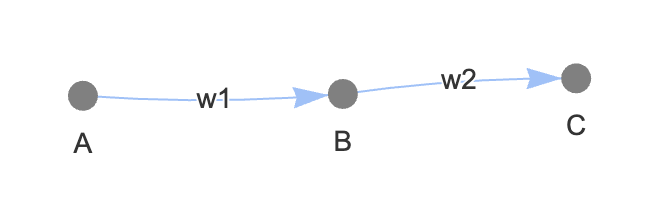
\includegraphics[width=0.4\textwidth]{delegation_graph_sample}
	\caption{Sample delegations}
	\label{fig:sample_delegations}
\end{figure}

As discussed in the previous section, resolving delegations happens iteratively, however, it is also possible to calculate a sink's final power recursively. When looking at the delegations in \cref{fig:sample_delegations}, we know, that sink C's power must be its own initial power of 1 in addition to $w_2$ times that of B, which in turn is one plus $w_1$ times that of A, etc. For a well formed delegation graph $G=(S\dot\bigcup D, E)$, we can define a node $v \in V$'s \textbf{standing power} as $p'_v = 1 + \sum_{(u, v, w) \in E} wp'_u$, from which we can create the following definition of final power of nodes:

\[
p_v = 
\begin{cases}
 p'_v v \in S \\ 
 0, v \in D 
 \end{cases}
\]

In order to find a sink node's standing power, knowledge of its delegator's standing power is necessary. However, since delegators definitively have a final power of zero, it is wrong to use their standing power value as their final power value. Instead, the standing power of a delegator can be ignored, and, assuming the delegation graph is well formed, its final power can be set to zero without further reflection. 

Given a directed, weighted delegation graph $G = (V = S \dot\bigcup D, E)$, the algorithm proceeds as follows.

\begin{enumerate}
\item Set up a system of linear equations, such that for each node $v \in V$ there is an equation $p'_v = 1+\sum_{(u, v, w) \in E}wp'_u$
\item Solve the system of linear equations to find the value of $p'_v$ for all $v \in V$
\item For each $s \in S$ set $p_s = p'_s$
\item For each $d \in D$ set $p_d = 0$
\end{enumerate}

In order to assure that the power is conserved during delegation, it may seem intuitive to add a constraint $\sum_{s \in S} p_s = |V|$ to the system of linear equations. However, we prove that such an equation is not strictly necessary, as the other equations in the system of equations already imply the conservation of power.

We start with the solutions $\{p'_v | v \in V\}$.

\begin{align*}
\forall v \in V: p'_v &= 1+\sum_{(u, v, w) \in E} \bigl(wp'_u \bigr) \\
\implies \sum_{v \in V} p'_v &= \sum_{v \in V} \bigl( 1 + \sum_{(u, v, w) \in E} \bigl( wp'_u \bigr ) \bigr) \\
&= \sum_{v \in V} 1 + \sum_{v \in V} \sum_{(u, v, w) \in E} wp'_u \\
&= |V| + \sum_{v \in V} \sum_{(u, v, w) \in E} wp'_u \\
&= |V| + \sum_{(u, v, w) \in E} wp'_u
\end{align*}

Focusing on the $\sum_{(u, v, w) \in E} wp'_u$ term, this can be re-grouped by $u$ as follows 

\begin{align*}
\sum_{(u, v, w) \in E} wp'_u &= \sum_{u \in V} \sum_{(u, v, w) \in E} wp'_u \\
&= \sum_{u \in V} p'_u  \sum_{(u, v, w) \in E} w
\end{align*}

Since, according to our definition of a delegation graph, all sinks have no outgoing notes, and all delegators's outgoing node weights add up to 1, we know that

\[
\sum_{(u, v, w) \in E} w = \begin{cases} 1, u \in D \\ 0, u \in S \end{cases}
\]

Thus, we can rewrite the above equation.

\begin{align*}
\sum_{u \in V} p'_u  \sum_{(u, v, w) \in E} w &= \left(\sum_{u \in D} p'_u  \sum_{(u, v, w) \in E} w \right) + \left( \sum_{u \in S} p'_u  \sum_{(u, v, w) \in E} w \right) \\
&= \left( \sum_{u \in D} p'_u \cdot 1 \right) + \left(\sum_{u \in S} p'_u \cdot 0 \right) \\
&= \sum_{u \in D} p'_u
\end{align*}

Focusing now on term $\sum_{v \in V} p'_v$, since $V = S \bigcup D$ , and $S$ and $D$ are disjunct we can say

\[
\sum_{v \in V} p'_v = \sum_{v \in S} p'_v  + \sum_{v \in D} p'_v 
\]

Thus, these two equations, we get

\[
\sum_{v \in S} p'_v  + \sum_{v \in D} p'_v  = |V| + \sum_{u \in D} p'_u
\]
\[
\implies \sum_{v \in S} p'_v   = |V| \qed
\]


\TODO{maybe prove correctness, but that would require some effort,}\\
\TODO{since we first need to establish what is "correct"}

\section{----------The one above was pasted in from my old "design" section, the stuff below is new, merge them------}

To explore the two approaches, they were implemented in Python. Python is versatile, simple, and offers a large collection of helpful libraries like NetworkX, a library for working with graphs \cite{hagbergExploringNetworkStructure2008}. 

The algorithms take as input python dictionaries ("dicts"), as inputs, which map a key to a value \cite{pythonsoftwarefoundationPythonTutorialSection}. The delegation graph is represented in a "dict of dicts" format, where every key in the outer dict is a node, and the value is another dict, which has the node's neighbors as keys, and a weight as value. The algorithm's use as input "inverse" delegation graphs, where the inner dictionaries represent a node's incoming delegations rather than its outgoing edges. \Cref{fig:inverse_dict_example} shows an example of this. This design choice improves efficiency, since the algorithms can directly look where each node gets its power form. This is particularly advantageous for the approach solving a system of linear equations, since the equations for a node's standing power are built based on its incoming delegations, not its outdoing delegations.

Despite all algorithm's taking in put in inverse dict-of-dicts format, there may still be preprocessing necessary. While the iterative solver can use the inverse dict-of-dicts directly, using it as a lookup table as it spreads power around the graph, the system of linear equations need to be constructed from the dict-of-dicts input. Including such set-up time in benchmarks may be misleading, as this time is not spent on actually resolving delegations, thus only the time spent actually resolving the delegations is used, and any set-up time is ignored. Nevertheless, in practice, the set-up time can be a relevant factor—depending on the use case and data format—when choosing between different approaches or implementations. The set-up procedures required for each implementation are described in more detail in the sections below.

\begin{figure}[t]
    \centering
    \begin{subfigure}[t]{0.45\textwidth}
        \centering
        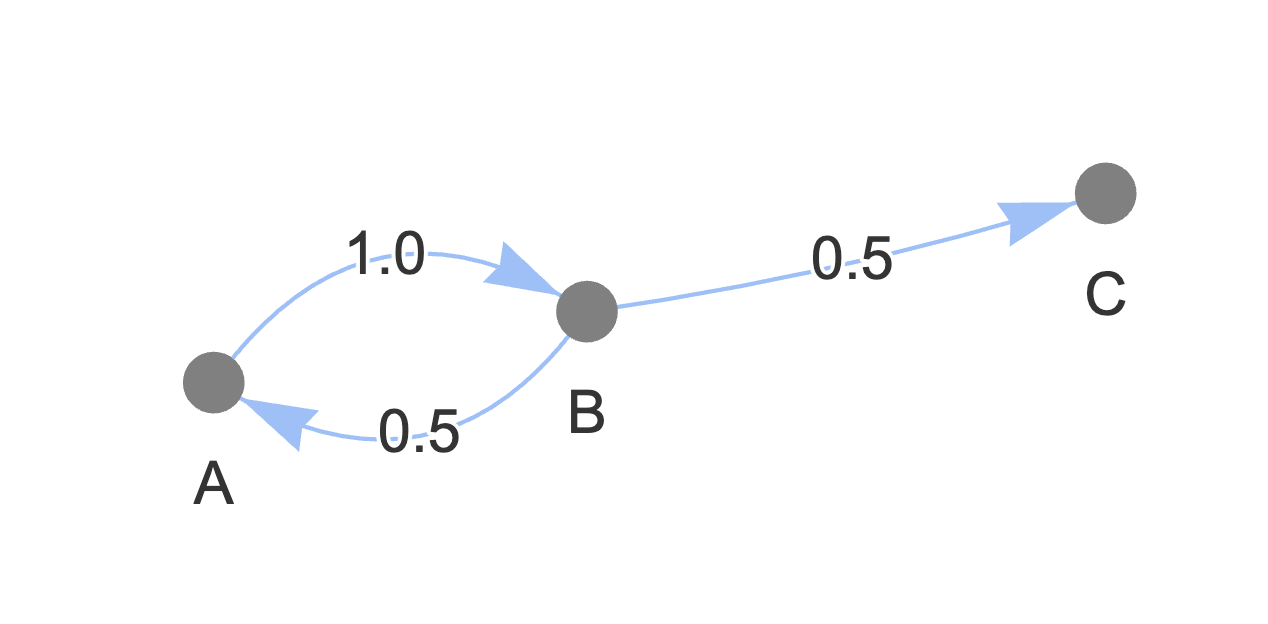
\includegraphics[width=\textwidth]{small_cycle_graph}
        \caption{Delegation graph}
    \end{subfigure}
    \hfill
    \begin{subfigure}[t]{0.45\textwidth}
        \centering
        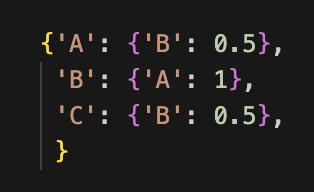
\includegraphics[width=\textwidth]{small_cycle_graph_inverse_dict}
        \caption{Inverse dict representation}
    \end{subfigure}
    \caption{Delegation graph and its inverse dict representation}
    \label{fig:inverse_dict_example}
\end{figure}

\section{Iterative Approach}

The implementation of the iterative approach is based closely on the pseudocode of \cref{alg:iterative_with_cutoff}. After initializing the power of all nodes to 1, the algorithm iteratively takes a snapshot of power values in the graph, and then distributes them according to the delegations, until the change in power each round falls below a cutoff value. 

The code takes the inverse dict-of-dicts representation of the delegation graph, a list of nodes, as well as a cutoff value as parameters, and returns the dict mapping nodes to their power values. The list of nodes must contain all the nodes in the graph since otherwise the code will not know about any nodes which have no incoming delegations. As discussed in \cref{sec:iterative_approach}, the cutoff value is necessary to ensure that the algorithm terminates in finite steps.

\section{System of Linear Equations Approach}

We try and compare two different approaches for resolving delegations using the systems of linear equations approach. Both delegations take as input an inverse dict-of-dicts representation of the delegations, as well as a list of nodes.

\subsection{Linear Programming Solver Implementation (LP Implementation)}

For this approach, we use the Python library PuLP, which provides an interface to Linear Programming (LP) solvers \cite{osullivanPuLPLinearProgramming2011}. To resolve the delegation graphs, we use the "Coin-or branch and cut" (CBC) solver, since it is free and open-source \cite{johnforrestCoinorCbcRelease2024}. Given the academic context and the moderate size of our delegation graphs, CBC provides a practical balance between performance and accessibility. Moreover, since our model essentially solves a system of linear equations with a unique correct solution, the choice of solver has little influence on the outcome itself — even if CBC is not the most optimized solver for this class of problems. While commercial solvers may offer faster runtimes, CBC is sufficient for our use case and ensures reproducibility without licensing constraints.

The algorithm first sets up the linear program, setting up an equation $p'_v = \sum_{(u, v, w) \in E} 1 + wp'_u$ for each node $v \in V$. This is then solved by the CBC solver, with the primal tolerance set to $5*10^{-3}$ to level the playing field compared to the iterative algorithm, which does not have perfect accuracy either. A tolerance of $5 * 10^{-3}$ assures that $\lvert p'_v -\sum_{(u, v, w) \in E} 1 + wp'_u \rvert \le 5*10^{-3}$, so the solutions will be correct when rounded to the second decimal place \cite{forrestCBCUserGuide2005}. Finally, the algorithm cleans the $p_v'$ values, setting any delegators power to 0. 

\subsection{Linear System Solver Implementation (LS Implementation)}

Secondly, we use a a dedicated linear system solver. We try SciPy's \texttt{scipy.sparse.linalg.spsolve} solver, which is optimized for sparse matrices \cite{virtanenSciPy10Fundamental2020}. A sparse solver is better equipped to resolve delegations if we assume that realistically each delegator only delegates to a few delegates. Since each $wp_v$ term in the system of linear equations can be mapped to one unique edge $(u, v, p) \in E$, the matrix corresponding to the system of linear equations likely has relatively few non zero entries compared to its size. In other words:

\[
\text{For a small } n \in \mathbb{N} \text{, and a large |V|}, D \subset V: n \cdot |D| < |V| \cdot |V|
\]

 \TODO{This explanation is ugly, but idk if its worth spending a lot more time on...} 
 
 The implementation makes use of SciPy's Compressed Sparse Column (CSC) arrays, which builds matrixes using $(x,y)$ coordinates and their corresponding data, which unless specified otherwise is 0 \cite{virtanenSciPy10Fundamental2020}. 

The solver solves the system of linear equations directly, using the SuperLU solver, so it is not possible to trade off runtime for accuracy, as done in the previous methods \cite{liSuperLUUsersGuide1999}. 

\TODO{Add links to the implementations on GitHub}

